%! Author = t.kramer
%! Date = 15/09/2024

\section{Research context}

% Research context
Indoor thermal comfort is strongly associated with occupant well-being \citep{altomonte_ten_2020}, overall satisfaction \citep{graham_lessons_2021} and energy use in buildings \citep{yang_thermal_2014}. As such, accurately projecting operational thermal comfort is a critical aspect of building design.

% Overview of current metrics
In the traditional building design workflow, thermal comfort assessments rely heavily on simulation data. This data forms the basis for calculating hourly thermal comfort indices, e.g., the Predicted Mean Vote (PMV). These indices are later aggregated into an annual, single-value metric (see \Cref{fig:typical-workflow}). Common long-term metrics derived from this approach include the \textit{Percentage of Time Outside a PMV Range} and the \textit{Percentage of Time Outside an Operative Temperature Range}, both featured in ISO-7730, EN-16798, and ASHRAE-55 \citep{iso_2005, cen_en_2019, ashrae_2020}. Other widely used metrics include the \textit{Degree Hours} method (ISO-7730, EN-16798) or the \textit{Average PPD} \citep{iso_2005}. Such metrics provide a broad, building-wide assessment of thermal comfort and are instrumental in guiding key design decisions regarding building form, envelope and particularly HVAC system design.

\begin{figure*}[h!]
    \centering
    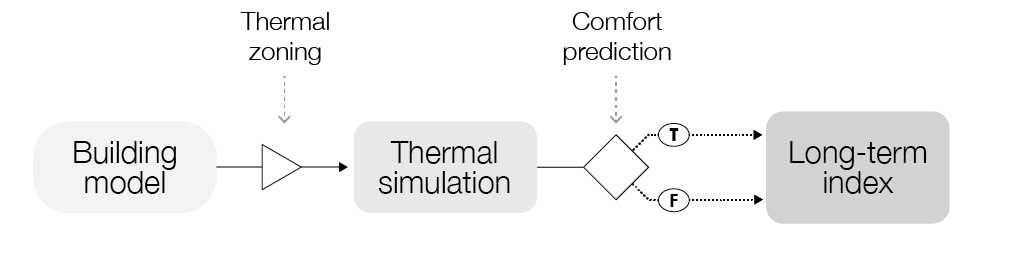
\includegraphics[width=10cm]{manuscript/src/figures/conventional-workflow.png}
    \caption{Traditional long-term thermal comfort prediction: Hourly simulated indoor climate data is assessed using a thermal comfort index (e.g. PMV) and is aggregated into a single value long-term (e.g. annual) metric. }
    \label{fig:typical-workflow}
\end{figure*}

% Critique 
Despite their widespread use, these traditional long-term thermal comfort metrics have inherent limitations.\citet{li_improved_2020} found that many of these metrics, including those featured in industry standards, show a weak correlation with actual thermal satisfaction among occupants.

Moreover, the most frequently used metrics rely on the Predicted Mean Vote (PMV) or Predicted Percentage Dissatisfied (PPD) models. Recent research has highlighted several problems of the PMV index: it often exhibits poor predictive accuracy \citep{cheung_analysis_2019}, advocates for excessively narrow temperature ranges \citep{arens_are_2010}, and is highly sensitive to personal input parameters such as clothing insulation and metabolic activity \citep{gauthier_role_2013}—variables that are hard to predict and often treated as constants in models \citep{carlucci_review_2012}, thus failing to represent real-world behavior accurately. Overall, these limitations tend to promote overly tight temperature ranges, which in turn leads to excessive energy use for space conditioning \citep{albatayneh_impact_2018, fukawa_field_2021, sekhar_thermal_2016}.

Several researchers have recognized these challenges and have proposed new long-term metrics in response. For example, based on continuous measurements and post-occupancy evaluations in air-conditioned office buildings, \citet{li_improved_2020} identified the \textit{percentage of time that daily temperature range exceeded a threshold} as the most effective index. The idea of using \textit{temporal exceedance} has been adopted earlier by others \citep{borgeson_comfort_2011, nicol_suggestion_2009}. Other suggestions include using the \textit{fraction of time within adaptive thermal comfort limits} \citep{albatayneh_development_2019}, \textit{adaptive degree-days} \citep{mcgilligan_adaptive_2011}, and \textit{overheating degree-days} \citep{estrella_guillen_comparing_2019}.

However, both new and conventional metrics share one substantial limitation: they typically capture only the temporal variability of thermal comfort while overlooking spatial differences within a thermal zone. This is a significant oversight, as recent studies have shown substantial spatial thermal heterogeneity within indoor environments \citep{mishra_thermal_2016, kramer_personal_2023}.
% Objective  
The objective of this paper is to introduce a new metric for comfort-based building performance assessment: spatial Thermal Autonomy (sTA). Compared to traditional metrics, sTA offers two significant advantages: (a) it accounts for spatial thermal variability, ensuring a more comprehensive evaluation of comfort throughout a building, and (b) it emphasizes energy-autonomous, passive building performance, reducing dependence on external energy sources.




